\section{Geometry}
\subsection{Line intersection}
\raggedbottom\lstinputlisting[style=cpp]{code/intersection.cpp}
\hrulefill
\subsection{Line and circle intersection}
\raggedbottom\lstinputlisting[style=cpp]{code/LineCircleIntersection.cpp}
\hrulefill
\subsection{Intersection of 2 circle}
\raggedbottom\lstinputlisting[style=cpp]{code/CirclesIntersection.cpp}
\hrulefill
\subsection{Convex hull 3D}
\raggedbottom\lstinputlisting[style=cpp]{code/ConvexHull3D.cpp}
\hrulefill
\subsection{Number of integer points inside polygon}
\raggedbottom\lstinputlisting[style=txt]{code/PointsInsidePolygon.txt}
\hrulefill
\subsection{Half plane}
\raggedbottom\lstinputlisting[style=cpp]{code/halfplane.cpp}
\hrulefill
\subsection{Is this point in circle of other 3 points?}
\raggedbottom\lstinputlisting[style=cpp]{code/point-in-circle.cpp}
\hrulefill
\subsection{Rotating Caliper}
\raggedbottom\lstinputlisting[style=cpp]{code/rotating-caliper.cpp}
\hrulefill
\subsection{Duality and properties}
duality of point (a, b) is y = ax - b and duality of line y = ax + b is (a, -b) \\
Properties:
\begin{enumerate}
    \item p is on l iff l* is in p*
    \item p is in intersection of l1 and l2 iff l1* and l2* lie on p*
    \item Duality preserve vertical distance
    \item Translating a line in primal to moving vertically in dual
    \item Rotating a line in primal to moving a point along a non-vertical line
    \item $li \cap lj$ is a vertex of lower envelope $\Longleftrightarrow$ (li*, lj*) is an edge of upper hull in dual
\end{enumerate}

\hrulefill
\subsection{Delaunay($nlg^2n$)}
\raggedbottom\lstinputlisting[style=cpp]{code/delaunay.cpp}
\hrulefill
\subsection{Stupid Delaunay($n^4$)}
\raggedbottom\lstinputlisting[style=cpp]{code/stupid-delaunay.cpp}
\hrulefill

\section{Graph}
\subsection{Maximum matching - Edmond's blossom}
\raggedbottom\lstinputlisting[style=cpp]{code/edmonds.cpp}
\hrulefill
\subsection{Biconnected components}
\raggedbottom\lstinputlisting[style=cpp]{code/bicon.cpp}
\hrulefill
\subsection{Gomory-hu}
\raggedbottom\lstinputlisting[style=cpp]{code/gomory-hu.cpp}
\hrulefill
\subsection{Directed minimum spanning tree (mlogn)}
\raggedbottom\lstinputlisting[style=cpp]{code/dmst_mlogn.cpp}
\hrulefill
\subsection{Directed minimum spanning tree (nm)}
\raggedbottom\lstinputlisting[style=cpp]{code/dmst_nm.cpp}
\hrulefill
\subsection{Dominator tree}
\raggedbottom\lstinputlisting[style=cpp]{code/dominator.cpp}
\hrulefill
\subsection{Flow - Dinic}
\raggedbottom\lstinputlisting[style=cpp]{code/flow.cpp}
\hrulefill
\subsection{Maximum weighted matching - Hungarian}
\raggedbottom\lstinputlisting[style=cpp]{code/hungarian.cpp}
\hrulefill
\subsection{Ear decomposition}
\raggedbottom\lstinputlisting[style=txt]{code/EarDecomposition.txt}
\hrulefill

\section{Combinatorics}
\subsection{LP simplex}
\raggedbottom\lstinputlisting[style=cpp]{code/simplex.cpp}
\hrulefill
\subsection{FFT}
\raggedbottom\lstinputlisting[style=cpp]{code/fft.cpp}
\hrulefill
\subsection{NTT}
\raggedbottom\lstinputlisting[style=cpp]{code/ntt.cpp}
\hrulefill
\subsection{Stirling 1}
\raggedbottom\lstinputlisting[style=cpp]{code/stirling.cpp}
\hrulefill
\subsection{Stirling 2}
$$ 
\left \{
  \begin{tabular}{c}
  n \\
  k
  \end{tabular}
\right \} = \frac{1}{k!}\sum_{j=0}^{k} (-1)^{k-j} \binom{k}{j} j^n
$$

\hrulefill
\subsection{Chinese remainder}
\raggedbottom\lstinputlisting[style=cpp]{code/chinese_remainder.cpp}
\hrulefill
\subsection{Popular LP}
{\Large BellmanFord:}\\
maximize $X_n$\\
$X_1 = 0$\\
and for eache edge ($v->u$ and weight w):\\
$X_u - X_v \le w$\\
\\
{\Large Flow:}\\
maximize $\Sigma f_{out}$ (where $out$ is output edges of vertex 1)\\
for each vertex (except 1 and n):\\
$\Sigma f_{in} - \Sigma f_{out} = 0$ (where $in$ is input edges of v and $out$ is output edges of v)\\  
\\
{\Large Dijkstra(IP):}\\
minimize $\Sigma z_i * w_i$\\
for eache edge ($v->u$ and weight w):\\
$0 \le z_i \le 1$\\
and for each ST-cut which vertex 1 is in S and vertex n is in T:\\
$\Sigma z_e \geq 1$ (for each edge e from S to T)\\
\\

\hrulefill
\subsection{Extended catalan}
number of ways for going from 0 to A with k moves without going to -B:
$$ \binom{k}{\frac{A+k}{2}} - \binom{k}{\frac{2B+A+k}{2}} $$

\hrulefill
\subsection{Find polynomial from it's points}
$P(x) = \sum_{i=1}^{n} y_i \prod_{j=1, j \neq i}^{n} \frac{x - x_j}{x_i - x_j}$

\hrulefill
\subsection{Number of primes}
\raggedbottom\lstinputlisting[style=txt]{code/NumberOfPrimes.txt}
\hrulefill
\subsection{Factorials}
\raggedbottom\lstinputlisting[style=txt]{code/Factorials.txt}
\hrulefill
\subsection{Powers of 3}
\raggedbottom\lstinputlisting[style=txt]{code/PowersOf3.txt}
\hrulefill
\subsection{C(2n,n)}
\raggedbottom\lstinputlisting[style=txt]{code/C_2n,n_.txt}
\hrulefill
\subsection{Most divisor}
\raggedbottom\lstinputlisting[style=txt]{code/MostDivisor.txt}
\hrulefill

\section{String}
\subsection{Manacher}
\raggedbottom\lstinputlisting[style=cpp]{code/manacher.cpp}
\hrulefill
\subsection{Palindromic tree}
\raggedbottom\lstinputlisting[style=cpp]{code/palindromic.cpp}
\hrulefill
\subsection{Z function}
\raggedbottom\lstinputlisting[style=cpp]{code/z.cpp}
\hrulefill

\section{Data structure}
\subsection{Treap}
\raggedbottom\lstinputlisting[style=cpp]{code/treap.cpp}
\hrulefill
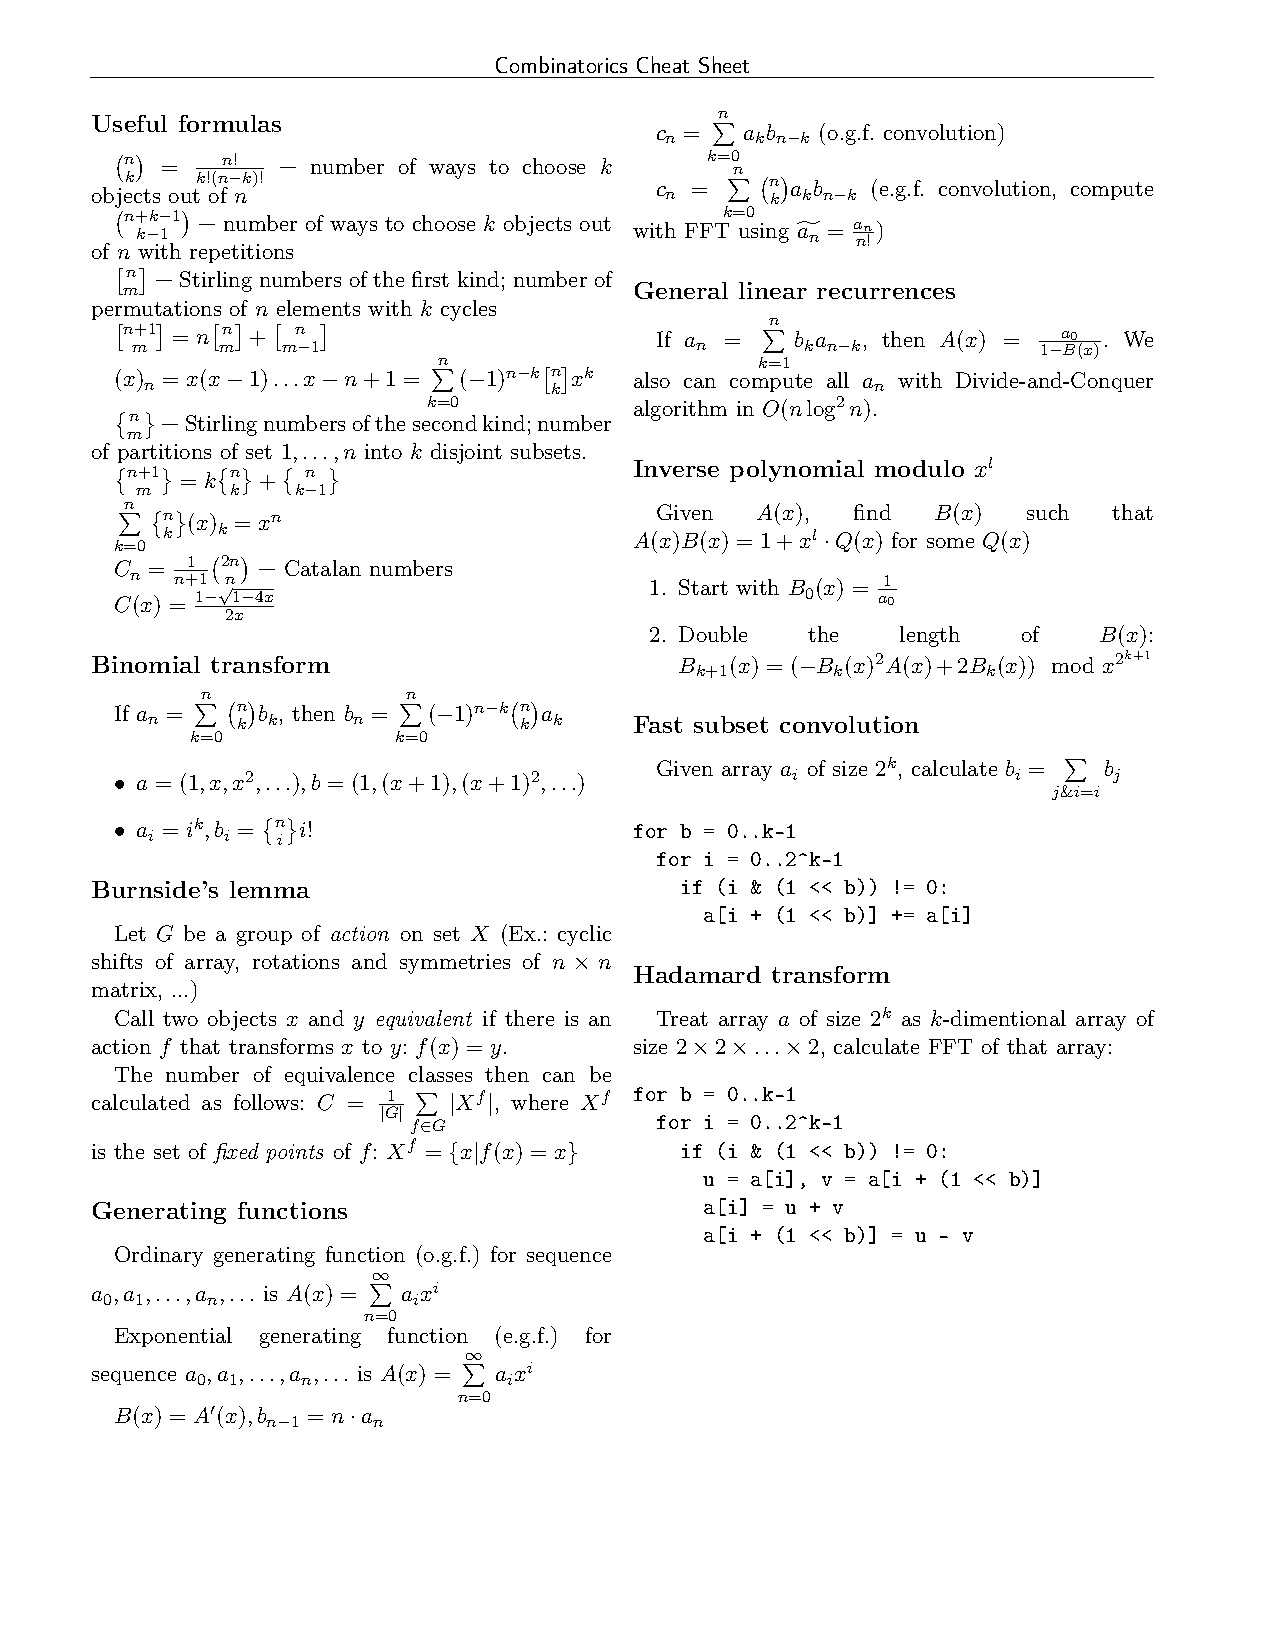
\includepdf[pages=-,pagecommand={\pagestyle{fancy}}]{code/Combinatorics.pdf}

